\section{Ejericio 5}
\subsection{Rutinas de atención de interrupciones}

En este punto, se nos encarga desarrollar las rutinas de atención de interrupciones para las distintas entradas de la IDT, en particular, la del reloj, la del telcado y la 0x46.\\

Como en este punto se nos pide el desarrollo de algunas funcionalidades que en los puntos posteriores son reemplazadas por otra, desarrollaremos en este punto el resultado final de las distintas rutinas, tal como se ven en el código terminado.\\

\subsubsection{Rutina de interrupción del reloj}

Cada vez que se llama a la interrupción del reloj ante cada tick, se llama a la función \texttt{sched\_tick}, quien realiza un llamado a game\_tick y además devuelve lo obtenido tras el llamado a \texttt{sched\_proxima\_a\_ejecutar} que es la próxima tarea a ejecutarse.\\

La función \texttt{game\_tick} llama a \texttt{screen\_actualizar} que pinta en pantalla los puntos de cada jugador, además de mostrar el reloj global del juego rotando, y el reloj particular del pirata actual, rotando debajo de su número indicador correspondiente, como indica la figura. Para los piratas no activos o muertos, se muestra una cruz.\\


\begin{figure}[ht]
\centering
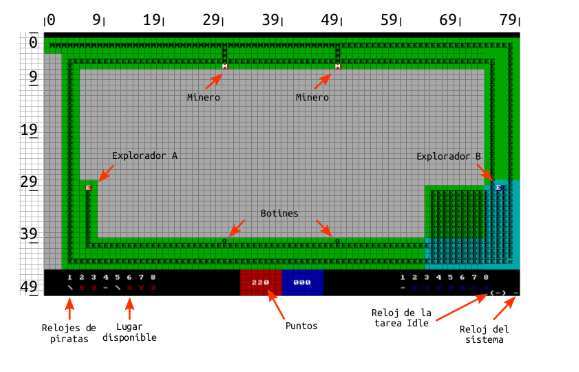
\includegraphics[width=90mm]{ej_5/img_ej_5.png}
\end{figure}


Además, si el jugador tiene mineros disponibles (es decir, tiene mineros para mandar, que se acumularon después de que un explorador descubriese un botín) y la cantidad de piratas vivos del jugador actual es menor a 8, se lanza un pirata minero con la función \texttt{game\_jugador\_lanzar\_pirata}. En esta función se inicializa un pirata a través de \texttt{game\_pirata\_inicializar} que primero busca cuál es el próximo id disponible para el pirata de un jugador, y luego inicializa los campos del struct pirata.\\

Después se inicializan las entradas de TSS y GDT correspondientes para el pirata a lanzarse con las funciones \texttt{tss\_inicializar\_pirata} y \texttt{gdt\_inicializar\_pirata} descritas en detalle en el punto siguiente y se pinta al pirata en pantalla con la función \texttt{screen\_pintar\_pirata}.
Luego actualizamos las variables del juego, aumentando la cantidad de piratas del jugador, y si el pirata lanzado es un explorador se aumenta la cantidad de exploradores del jugador actual.\\

Si es minero cambiamos el cr3 actual por el cr3 del minero obtenido de su TSS para obtener del stack del minero las direcciones destinadas a botín x e y, y las actualizamos con la posición del botín del jugador.
Finalmente, se restaura el viejo cr3 y decrementa en uno la cantidad de mineros disponibles del jugador, ya que ahora tiene uno menos para mandar.\\


En la función \texttt{sched\_proxima\_a\_ejecutar} utilizamos la función auxiliar \texttt{sched\_proximo\_pirata}, que recibe un id de jugador y id de pirata y se fija para ese jugador, cual es el siguiente al pirata dado que está vivo y lo devuelve. En caso de que no haya ninguno, se devuelve -1.\\

Luego, se chequea, en primer caso, si no hay ninguna tarea activa para ningún jugador (es decir, el llamado para \texttt{game\_proximo\_pirata} para ambos jugadores con el pirata actual dio -1), devuelve el índice en GDT de la tarea Idle.\\

Sino, se llama a \texttt{game\_proximo\_pirata} con ambos jugadores y el pirata actual y se determina para cada jugador, cual es el próximo pirata a ejecutarse, en caso de que tenga uno, y se setea la proxima tarea a ejecutarse según cual sea el jugador actual (en este caso, la siguiente del otro jugador) o según el otro jugador no tenga tareas para ejecutar (en este caso, la siguiente del jugador con tareas). \\

Finalmente, con lo devuelto por \texttt{sched\_tick} (el indice en GDT de la próxima tarea a ejecutarse) seteamos el valor del selector en [sched\_tarea\_selector] y realizamos un jmp far a [sched\_tarea\_offset] definidos previamente como sched\_tarea\_offset: dd 0x00 sched\_tarea\_selector: dw 0x00 en la sección de datos, completando el task switch.\\

\subsubsection{Rutina de atención del teclado}

Para la atención del teclado, en la rutina leemos la tecla que fue presionada y con esta llamamos a \texttt{game\_atender\_teclado}, que en caso de recibir la tecla Shift Left o Shit Right lanza al pirata correspondiente. Además, en caso de que sea la tecla Y, setea el modo debug según corresponda.\\

\subsubsection{Rutina de atención de las syscalls (\_isr70)}

En la rutina \texttt{\_isr70} llamamos a la función \texttt{game\_syscall\_manejar} con el número de syscall recibida, para luego realizar las distintas rutinas según sea necesario. Las distintas rutinas son:

\begin{enumerate}

	\item \texttt{game\_syscall\_pirata\_mover} que recibe como parámetros un id de pirata y una dirección a la cual debe moverse, que se basa en un enum que tiene los valores ABA, ARR, IZQ, DER.
	Para poder manejar la dirección pasada como parámetros de la misma forma en la que tratamos a las coordenadas de los piratas, convertimos la dirección a un struct coord con la función \texttt{game\_dir2coord}. Una vez realizada la conversión, con la función \texttt{game\_posicion\_valida}, comprobamos que la posición a la que queremos movernos esté dentro de los límites del mapa. Si no lo está, retornamos sin realizar ningún movimiento. Caso contrario, actualizamos la posición del pirata. Si el pirata es explorador, y la posición no había sido previamente explorada por éste, llamamos a \texttt{game\_habilitar\_posicion} que es una función que para cada posición alrededor del explorador, incluyendo a la actual, si ésta no fue explorada la marca como explorada y la mapea. Además, chequea si hay tesoro en esa posición, y de ser así, incrementa en uno la cantidad de mineros del jugador ya que en el próximo \texttt{game\_tick} deberá lanzarse un minero. Además se guarda en el botín del jugador la coordenada recién habilitada.


	\item \texttt{game\_syscall\_cavar} recibe un id de pirata. Si este no corresponde a un minero, retornamos sin realizar ninguna acción.
	Si es minero, llamamos a \texttt{game\_buscar\_botin} con el pirata para ver si en la posición dada hay un botin. Si lo hay pero el valor del tesoro, calculado con \texttt{game\_valor\_tesoro} es 0, se libera al minero, mientras que si el valor es mayor a 0, se suma uno a la cantidad de monedas del jugador que mando la syscall y se resta uno al botín de la posición.

	\item \texttt{game\_syscall\_pirata\_posicion} recibe como parámetro el id del pirata que llama a la syscall y el id del pirata del cuál se quiere conocer la posición. Si el id del pirata del cual se quiere conocer la posición es -1, se devuelve la posición del jugador que llama a la syscall, caso contrario, se devuelve la posición del pirata cuyo id fue pasado por parámetro.

\end{enumerate}
